\chapter{Observations}
\label{chap:observations}

The data presented in this thesis are part of an ALMA survey of Orion proplyds in Orion (project 2011.0.00028.S); data collection and analysis methods of the continuum results are presented in \citep{mann_alma_2014}. Since this was part of a Cycle 0 Early Science project, the survey used only 22 of the array's 12 meter dishes in a hybrid configuration, with baselines ranging from 21.2 to 384.2 meters, yielding maximum angular scales and angular resolution of 8" and 0."5, respectively. At a distance of 389 pc for the distance to these sources, max angular scales and angular resolution correspond to 3,112 AU and 194 AU, respectively. The distance to the stars used here was recently measured by GAIA (\citep{gaia_collaboration_gaia_2016}, \citep{gaia_collaboration_gaia_2018}) to be 389 \pm 7.97, nearer than the previous measurement of 414 pc.
% sig figs on the distance
% For Gaia references: https://gea.esac.esa.int/archive/documentation/GDR2/bib.html#bib173

Observations were made in Band 7 in four 1.875 GHz-wide bands arranged to cover the rest frequencies of the HCO+ (4-3), HCN (4-3), CO (3-2), and CS (7-6) transitions (356.734 GHz, 354.505 GHz, 345.796 GHz, and 342.883 GHz, respectively). Each band was split into 3840 channels with width 488.28 kHz, yielding a velocity resolution of 0.42 km s$^{-1}$.



Analysis showed that excluding baselines shorter than 110 k$\lambda$, 80 k$\lambda$, and 60 k$\lambda$ for HCO$^{+1}$, HCN, and CO respectively optimized signal-to-noise ratios for each data set. The CS line showed no improvement with baseline cutting. These cuts resulted in decreased maximum recoverable angular scales of 1, 2, and 3.

% Maybe put an image of HCO+ before and after the cuts here?
\begin{figure}
\centering
\begin{minipage}{.5\textwidth}
  \centering
  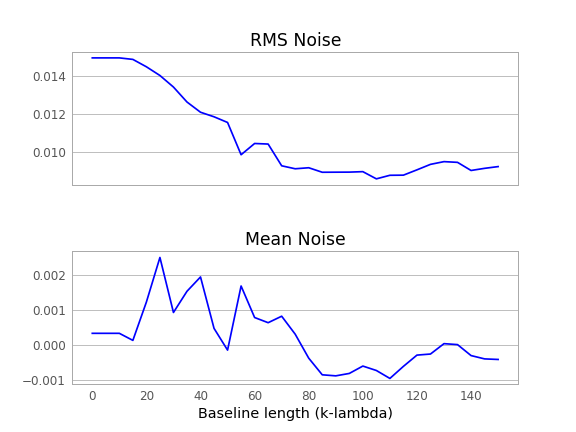
\includegraphics[width=.4\linewidth]{hcn-imnoise_hcn10000.png}
  \captionof{figure}{A figure}
  \label{fig:test1}
\end{minipage}%
\begin{minipage}{.5\textwidth}
  \centering
  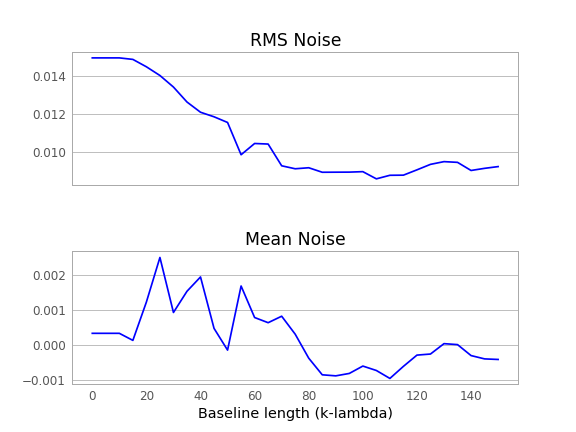
\includegraphics[width=.4\linewidth]{hcn-imnoise_hcn10000.png}
  \captionof{figure}{Another figure}
  \label{fig:test2}
\end{minipage}
\end{figure}

These data, from Field 4 of Mann et al (2014) (citation) represent 13.6 minutes of on-source time. This duration was split into six 136 second observations, spaced out over 7.5 hours to ensure adequate \textit{uv} coverage, resulting in a synthesized beam of 0."57 $\cross$ 0."51 with a position angle of PA. Precipitable water vapor in the atmosphere was stable at 0.7 mm.




The data were calibrated by ALMA staff using standard procedures in the Common Astronomy Software Applications (CASA, citation). The antenna-based complex gains and bandpass response of the system were calibrated using observations of the quasars J0607-085 and J0522-364 respectively. The ab- solute flux calibration was determined from observations of Callisto. The model of Callisto was drawn from Butler (2012) (citation). Absolute flux calibration is estimated to be accurate to within ∼ 10\% (Mann et al. 2014).

The velocity reference frame was converted from CASA's standard topocentric frame to LSRK (kinematic local standard of rest) using the CASA task cvel. Next, continuum emission was subtracted in the uv plane using the CASA task contsub. Visibilities were then inverted with natural weighting, deconvolved, and restored using standard procedures from the Multichannel Image Reconstruction Image Analysis and Display, or MIRIAD, package (Sault et al. 1995) (citation)








\iffalse
Things to get:
* noise profiles as func of baseline
* Noise levels
* Beam size, max angular scales after baseline cuts (how to get that?)
* Beam position angle
* Does ICR use natural weighting? (using robust=2)
\fi
% Note that no closing info is needed.
